%%% DOCUMENT BEGIN

\documentclass{article}

\usepackage[utf8]{inputenc}

\usepackage{geometry}
\geometry{a4paper}

\usepackage{graphicx}

%%% PACKAGES
\usepackage{booktabs} % for much better looking tables
\usepackage{array} % for better arrays (eg matrices) in maths
\usepackage{paralist} % very flexible & customisable lists (eg. enumerate/itemize, etc.)
\usepackage{verbatim} % adds environment for commenting out blocks of text & for better verbatim
\usepackage{subfig} % make it possible to include more than one captioned figure/table in a single float

%%% HEADERS & FOOTERS
\usepackage{fancyhdr} % This should be set AFTER setting up the page geometry
\pagestyle{fancy} % options: empty , plain , fancy
\renewcommand{\headrulewidth}{0pt} % customise the layout...
\lhead{}\chead{}\rhead{}
\lfoot{}\cfoot{\thepage}\rfoot{}

%%% SECTION TITLE APPEARANCE
\usepackage{sectsty}
\allsectionsfont{\sffamily\mdseries\upshape}

%%% ToC (table of contents) APPEARANCE
\usepackage[nottoc,notlof,notlot]{tocbibind} % Put the bibliography in the ToC
\usepackage[titles,subfigure]{tocloft} % Alter the style of the Table of Contents
\renewcommand{\cftsecfont}{\rmfamily\mdseries\upshape}
\renewcommand{\cftsecpagefont}{\rmfamily\mdseries\upshape} % No bold!


%%% END Article customizations


%%%%%%%%%%%%%%%%%%%%%%%%%
%%%          Fill in the title details                      %%%

\def \thetitle {INF-1400 Object oriented programming}
\def \thesubtitle {Assignment 3 - Mayhem clone}
\def \theauthor {Marius Mæland and Raymon S. Hansen}
\def \pagecount {3}

%%%%%%%%%%%%%%%%%%%%%%%%%

%\pagestyle{fancy}
\pagestyle{fancyplain} % options: empty , plain , fancy
\renewcommand{\headrulewidth}{1pt} % customise the layout...
\renewcommand{\footrulewidth}{0pt}
\lhead{\fancyplain{}{\thetitle{} -- \thesubtitle{}}}\chead{}\rhead{\fancyplain{}{\theauthor{}}}
\lfoot{}\cfoot{Page {\thepage} of \pagecount}\rfoot{}

\begin{document}

%%% TITLE PAGE

\begin{titlepage}
\begin{center}



\textsc{\\[3.5cm] \huge University of Tromsø}\\[1.5cm]

\textsc{\LARGE \thetitle}\\[0.5cm]

\textsc{\Large \thesubtitle}\\[1.5cm]

\LARGE{\theauthor} \\[0.5cm] \large{Department of Computer Science}



\vfill
{\large \today}

\end{center}
\thispagestyle{empty}
\end{titlepage}

\newpage{}


%%% TABLE OF CONTENTS

%\tableofcontents


\newpage{}

%%% DOCUMENT BODY

%%% Set counter to 1
\setcounter{page}{1}

\section{Introduction}

Short introduction to the assignment, motivation and expected results.\\

The assignment is to implement a clone of the old game Mayhem, but in this case we ended up with a space shooter death match type of game, however all of the requirements of the assignment are met. 

\subsection{Requirements}

Outline the detailed requirements specified in the assignment text. \\

Requrements for this assignment is to create a multiplayer game where each player can control their spaceship with four buttons, when thrusting the spaceships should move in the direction it is pointing, and are to be rotated right or left to control where to go. The ships should also be able to fire bullets.\\

Other requirements for the game:

\begin{itemize}

\item Two space ships
\item Four controls for each player
\item Controls: rotate left, rotate right, thrust and fire
\item Minimum one obstacle
\item Spaceship can crash with other objects on the screen
\item Gravity that acts on spaceships
\item A score for each player displayed on screen
\item Limited amount of fuel to the spaceships
\item Refuel station/ refuel pick up

\end{itemize}

There are also some requirements for the code:

\begin{itemize}

\item The code should be split in minimum two files
\item The main loop must have timing
\item The game shall be started using: 
\begin{verbatim} if__name__ == '__main__':\end{verbatim}
\item All visible objects shall subclass the pygame.sprite.Sprite class
\item All modules, classes and methods shall contain docstrings

\end{itemize}

\section{Technical Background}

Which topics are covered in this assignment. Should be short and cover the necessary topics without mentioning your specific implementation and design.\\

One of the requirements was that all moving objects in the game should sub-class
pygames sprite module. The pygame Sprite module is designed to make simple game 
design easier for developers. It includes built in functions for referring to 
and working with coordinates, displaying images for a better graphical look as
well as detecting collisions and working with objects/sprites in groups. 

Sprite groups is practical because it makes the use of polymorphism very easy.
The sprite module has a built in draw function which blits each sprites "image" 
attribute on a surface. We have also used this to simplify per frame update calls
on many different objects.

Allthough not a specific requirement, we have implemented and thoroughly enjoyed 
making animations with sprite sheets. Linking the actual code and the image 
files has given us valuable insight into how code interacts with "the outside world".
Cutting specific sections of a sprite sheet proved difficult at times, as each sheet
had a different layout, size, padding, alpha channels etc. 


\subsection{Data Structures}

Since this is a course in algorithms, so it might be a good idea to cover the basic data-structures(e.g. lists and trees). 

Figure \ref{fig:ackseq} shows how you can add figures to the report. And below is the LaTeX syntax for adding a figure:

% Verbatim prints the text without formatting
\begin{verbatim}
\begin{figure}
\begin{center}
\fbox{\includegraphics[width=177px]
{source.png}}
\end{center}
\caption{Description}\label{fig:descriptiveLabel}
\end{figure}
\end{verbatim}

% An example figure
\begin{figure}[h]
\begin{center}
\fbox{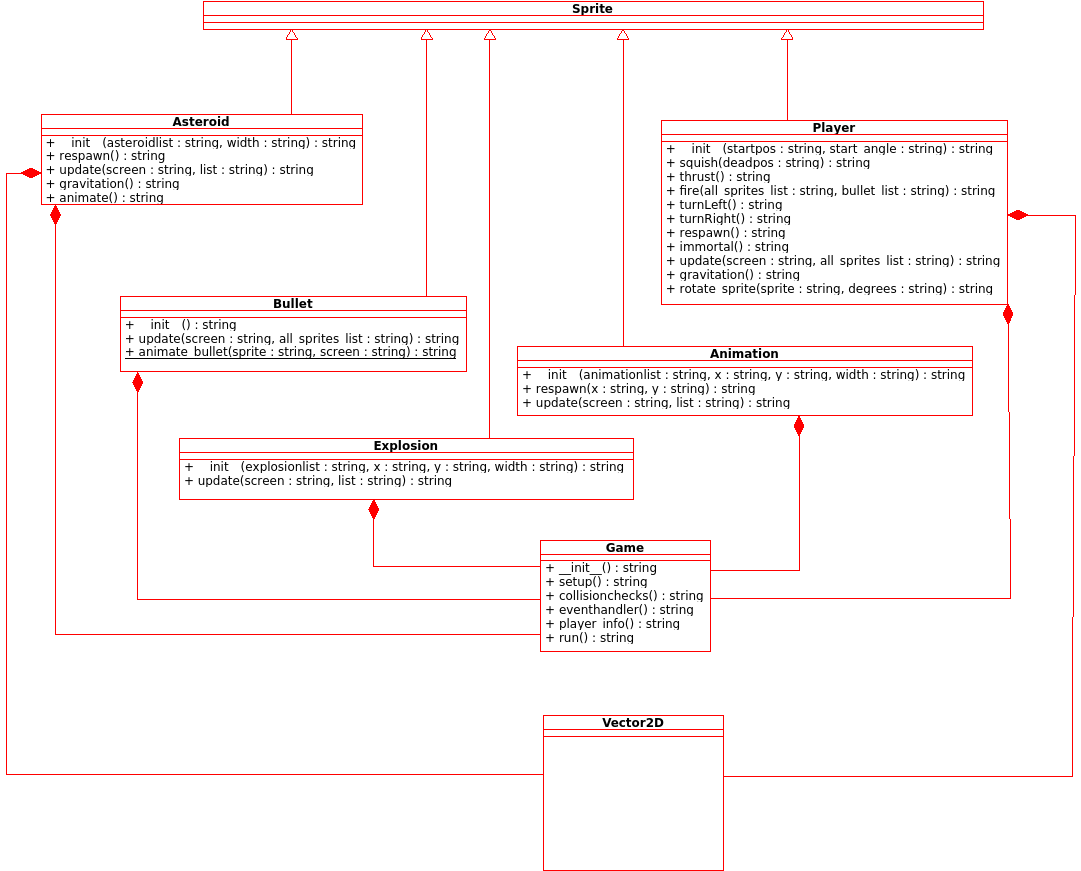
\includegraphics[width=177px]
{classdiagram.png}}
\end{center}
\caption{A binary search tree}\label{fig:ackseq}
\end{figure}

\subsection{Another section}

Some more information

\section{Design}

How did you solve the assignment? Describe the architecture and any design choices you've made. Show figures of the proposed architecture.

\section{Implementation}

How did you implement, deploy and run your application? No need to refer to actual lines of code.

\section{Discussion}

Any advantages or disadvantages with your design?

\subsection{Evaluation}

This section should contain relevant graphs and test results.

\section{Conclusion}

Sum up by restating the problem and solution. Follow up with a brief summary of the solution along with lessons learned.


%%% BIBLOGRAPHY

\newpage{}


\begin{thebibliography}{9}

\bibitem{coursebook}
 Robert Sedgewick 
  \emph{Algorithms in C - parts 1-4}.
  Addison-Wesley Publishing Company,
  3. Edition,
  1998.

\end{thebibliography}

\end{document}
